\section{Architektur}

\begin{figure}[ht]
	\centering
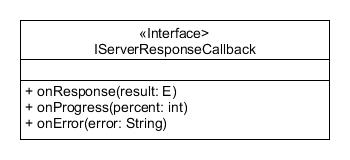
\includegraphics[width=1\textwidth]{./resources/Diagramme/App/UMLAndroidApp.jpg}
\caption{UML Diagram der Android App}
	\label{fig:modules_overview}
\end{figure}

\subsection{Entwurfsmuster}
In der App werden Entwurfsmuster verwendet, um Komponenten leicht austauschen zu können und um die Nutzeroberfläche und den Funktionsumfang einfach erweitern zu können. Der Einsatz von Entwurfsmustern Verhindert  zudem, dass Klassen einer Schicht Zugriff auf die Klassen der Übernächsten Schicht haben müssen und reduziert die Aufrufe von Klassen einer niederen Schicht auf die darüber liegende Schicht.

\subsubsection{Facade}
Das Facade Muster ist bei der Klasse \nameref{app:klasse:LogInHelper} zu sehen. Sie vereinfacht die Überprüfung, ob eine Nutzer bereits eingeloggt ist und verhindert, dass die View-Schicht direkt auf die Model-Schicht zugreifen muss.

\subsubsection{Observer}
Das Observer Muster reduziert die Aufrufe von Klassen einer niederen Schicht auf die darüber liegende Schicht, wie es das \nameref{app:klasse:IRecordCallback}, das \nameref{app:klasse:IPersistCallback} und das \nameref{app:klasse:IServerResponseCallback} tun. Nützlich ist das Observer Muster vor allem dann, wenn ein asynchroner Task ausgeführt wird und der Aufrufer erst benachrichtigt werden soll, wenn dieser Task zu Ende ist.\newline
Bei der Umsetzung des Observer Musters weicht die App von der herkömmlichen Art ab: Während normalerweise eine Klasse, die als Observer agiert, das Interface, also einen der Callbacks, implementiert, hat in der App im Gegensatz dazu eine Klasse ein Attribut vom Typ des jeweiligen Interfaces. Bei der Instanziierung dieses Attributes findet die Implementierung des Interfaces statt.

\subsubsection{Command}
Das Command Muster kommt bei jedem asynchronen Task zum einsatz. In den Konstruktoren der Tasks wird der Command erstellt, durch die \textit{start} Methode wird der Command ausgeführt. Somit muss sich keine Komponente um die eigentliche Ausführung langwieriger Operationen kümmern.

\subsubsection{Proxy}
Das Proxy Muster kommt zum Einsatz, sobald Anfragen an den Server gesendet werden oder Operationen auf dem Speicher ausgeführt werden sollen. Die entsprechenden Klassen sind \nameref{app:klasse:ServerProxy} und \nameref{app:klasse:MemoryManager}. Dadurch muss keine der Klassen, die den ServerProxy oder den MemoryManager verwenden über die zugrunde liegende Infrastruktur und deren Handhabung bescheid wissen.

\subsubsection{Template Method}
Das Template Method Muster, zu Deutsch ``Schablonenmethode'', findet seinen Einsatz in der \nameref{app:klasse:ContainerActivity}. Die ContainerActivity ist eine Activity, die immer nachd dem gleichen Schema aufgebaut ist: Eine Toolbar am oberen Bildschirmrand und ein Fragment mit dem Inhalt darunter. Sie selbst lädt immer die gleiche Ansicht, lässt aber ihre Unterklasse bestimmen, welches Fragment angezeigt wird. Dadurch können ohne großen Aufwandt witere Ansichten eingefügt werden. Der einzige Aufwandt besteht im erben von ContainerActivity und dem Implementieren der \textit{selectFragment} Methode.\newline
Sollte später eine Activity mit einem ViewPager eingefügt werden, der beispielsweise Aufgenommene und Heruntergeladene Videos in eigenen Tabs anzeigen kann, bietet sich die Schablonenmethode wieder an: In diesem Fall gäbe es eine Acitivty, die ein Layout lädt, welches über einen ViewPager verfügt. Die Unterklassen bestimmen dann auf welcher Seite welches Fragment eingeblendet wird. Natürlich müsste die Nummer des aktuellen Tabs des ViewPagers in der \textit{selectFragment} Methode mitgeliefert werden.

\subsubsection{Strategy}
Die Strategy Methode kommt in den Klassen \nameref{app:klasse:CameraHandler}, \nameref{app:klasse:IFileEncryptor} und \nameref{app:klasse:IKeyEncryptor}  zum Einsatz. Sie ermöglicht die Austauschbarkeit der Kameraimplementierung bzw. der Verschlüsselungsalgorithmen und macht ihre Klienten nur von den Schnittstellen abhängig.
